\documentclass{article}

\usepackage{geometry}
\usepackage{xeCJK}
\usepackage{amsmath}
\usepackage{tikz}
\usepackage{pgfplots}
% figure[H] float
\usepackage{float}
\usepackage{amssymb}
\usepackage{hyperref}
\usepackage{setspace}
% 修改公式编号
\usepackage{chngcntr}

% 设置行间距 1.5 倍
\renewcommand{\baselinestretch}{1.5}
% 自定义图片的标题:Figure -> 图
\renewcommand{\figurename}{图}

% 设置页大小和页边距,或者scale=0.8
\geometry{a4paper,left=3.18cm,right=3.18cm,top=2.54cm,bottom=2.54cm}
% 兼容
\pgfplotsset{compat=1.16}
% 中文默认没有斜体和粗体格式,开启伪斜体和指定黑体;
\setCJKmainfont[AutoFakeSlant, BoldFont=SimHei]{SimSun}
\usetikzlibrary{positioning}
\hypersetup{
    colorlinks,
    citecolor=black,
    filecolor=black,
    linkcolor=black,
    urlcolor=black
}
% 每个章节后,重置公式编号
\counterwithin*{equation}{section}

\begin{document}
  \tableofcontents
  \newpage

  \part{函数与极限}
  \section{集合}
    \subsection{表示法}
\begin{enumerate}
  \item 列举法:$A = \{a_1, a_2, ..., a_n\}$
  \item 描述法:$M = \{x | \text{x具有性质P} \}$
\end{enumerate}

\subsection{数集}
\paragraph{}
在字母右上角标 “*”,表示排除 0 元素的数集;
\paragraph{}
在字母右上角标 “+”,表示排除 0 元素与负数的数集。
\paragraph{}
例子:自然数集 N 和整数集 Z

\begin{gather}
N^* = \{1, 2, ..., n, ...\} \\
Z^+ = \{1, 2, ..., n, ...\}
\end{gather}

\subsection{集合关系}
\paragraph{}
子集、真子集、相等、空集(是任何集合的子集)

\subsection{集合运算}
\paragraph{}
并、交、差(\textbackslash)
\paragraph{}
差运算;如果 I 是全集(基本集),也相当于求 A 的补集(余集):

\begin{equation}
I \backslash A = A^c = \{x | x \in I, x \notin A\}
\end{equation}

\paragraph{}
$A^c$ 是补集

\subsubsection{法则}
\begin{enumerate}
  \item 交换律:
    \begin{enumerate}
      \item $A \cup B = B \cup A$
      \item $A \cap B = B \cap A$
    \end{enumerate}
  \item 结合律:
    \begin{enumerate}
      \item $(A \cup B) \cup C = A \cup (B \cup C)$
      \item $(A \cap B) \cap C = A \cap (B \cap C)$
    \end{enumerate}
  \item 分配律:
    \begin{enumerate}
      \item $(A \cup B) \cap C = (A \cap C) \cup (B \cap C)$
      \item $(A \cap B) \cup C = (A \cup C) \cap (B \cup C)$
    \end{enumerate}
  \item 对偶律:
    \begin{enumerate}
      \item ${(A \cup B)}^c = A^c \cap B^c$
      \item ${(A \cap B)}^c = A^c \cup B^c$
    \end{enumerate}
\end{enumerate}

\subsubsection{直积}
\begin{equation}
A \times B = \{(x, y) | x \in A, y \in B\}
\end{equation}

\subsection{区间和邻域}

\subsubsection{区间}
\paragraph{}
(a, b)、[a, b]、[a, b)、(a, b]
\subsubsection{邻域}

\paragraph{}
邻域:
\begin{equation}
U(a, \delta) = \{x | a - \delta < x < a + \delta\}
\end{equation}

\paragraph{}
去心邻域:
\begin{equation}
\mathring{U}(a, \delta) = \{x | 0 < |x - a| < \delta\}
\end{equation}

  \section{映射}
    \begin{enumerate}
  \item 非空集合 $X, Y$
  \item 法则 $f$
  \item $X$ 中的每个元素 $x$,在法则 $f$ 下,能从 $Y$ 中找到\textbf{唯一}的值 $y$ ,即: $y = f(x)$
\end{enumerate}

\begin{equation}
f:X \to Y
\end{equation}

\paragraph{}
x与y关系:一对一、多对一


\begin{figure}[H]
\centering
  %------- 第1行 -------
  \begin{subfigure}[t]{0.4\linewidth}
    \centering
      % x 与 y 关系,一对一
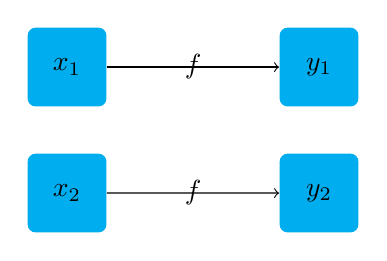
\begin{tikzpicture}[scale=0.8]
  \node [fill=cyan,minimum size=1cm,rounded corners=.1cm]   (x1) at (0,0)    {$x_1$};
  \node [fill=cyan,minimum size=1cm,rounded corners=.1cm]   (x2) at (0,-2)   {$x_2$};
  \node [fill=cyan,minimum size=1cm,rounded corners=.1cm]   (y1) at (4,0)   {$y_1$};
  \node [fill=cyan,minimum size=1cm,rounded corners=.1cm]   (y2) at (4,-2)   {$y_2$};

  \draw [->] (x1) -- (y1) node[midway] {$f$};
  \draw [->] (x2) -- (y2) node[midway] {$f$};
\end{tikzpicture}

      \caption{一对一}
  \end{subfigure}
  \begin{subfigure}[t]{0.4\linewidth}
    \centering
      % x 与 y 关系,多对一
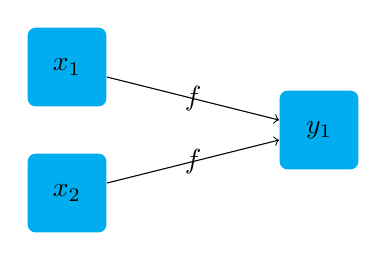
\begin{tikzpicture}[scale=0.8]
  \node [fill=cyan,minimum size=1cm,rounded corners=.1cm]   (x1) at (0,0)    {$x_1$};
  \node [fill=cyan,minimum size=1cm,rounded corners=.1cm]   (x2) at (0,-2)   {$x_2$};
  \node [fill=cyan,minimum size=1cm,rounded corners=.1cm]   (y1) at (4,-1)   {$y_1$};

  \draw [->] (x1) -- (y1) node[midway] {$f$};
  \draw [->] (x2) -- (y1) node[midway] {$f$};
\end{tikzpicture}

      \caption{多对一}
  \end{subfigure}
  \caption{x 与 y 关系}
\end{figure}

\paragraph{}
\textbf{概念}

\begin{enumerate}
  \item 定义域(Domain):$D_f = X$
  \item 值域(Range):$R_f = Y = f(x)$
\end{enumerate}

\begin{enumerate}
  \item 满射:$Y$ 中任意一个元素 $y$,都是 $X$ 中某一元素的像
  \item 单射:$X$ 中任意两个元素 $x_1 \neq  x_2$,它们的像不一样,$f(x_1) \neq  f(x_2)$
  \item 双射(一一映射):满足单射和满射条件
\end{enumerate}

\subsection{逆映射}

\begin{enumerate}
  \item $f$ 是 $X$ 到 $Y$ 的单射
  \item 则逆映射 $f^{-1} = g$,值域 $R_f$ 到 $X$ 的映射,即 $g(y) = x$
\end{enumerate}

\begin{equation}
g:R_f \to X
\end{equation}

\subsection{复合映射}

\begin{enumerate}
  \item 设有两个映射 $g:X \to Y_1$,$f:Y_2 \to Z$
  \item $Y_1 \subset Y_2$
  \item 则 $X$ 到 $Z$ 的映射,记作:$f \circ g$
\end{enumerate}

\begin{gather}
f \circ g: X \to Z \\
(f \circ g)(x) = f[g(x)], x \in X
\end{gather}

  \section{函数}
    \subsection{函数}
\paragraph{}
在数集上的映射,$D \subset R$,$f:D \to R$ 称为函数。

\subsection{函数的表示}

\begin{enumerate}
  \item 表格法
  \item 图形法
  \item  解析法(公式法)
\end{enumerate}

\subsection{函数的特性}

\subsubsection{有界性}

\begin{enumerate}
  \item 上界:存在数 $K_1$,满足 $\forall{x},\ f(x) \leq K_1$
  \item 下界:存在数 $K_2$,满足 $\forall{x},\ f(x) \geq K_2$
  \item 有界:存在正数 $M$,满足 $\forall{x},\ |f(x)| \leq M$
  \item 无界:不存在 $M$ 使得第 3 点的公式成立
\end{enumerate}

\subsubsection{单调性}
\paragraph{}
在区间上的单调性:设函数 $f(x)$ 的定义域为 $D$ ,在区间 $I \subset D$ 上的任意两点 $x_1, x_2$,且 $x_1 < x_2$,恒有:

\begin{enumerate}
  \item 单调增加:$f(x_1) < f(x_2)$
  \item 单调减少:$f(x_1) > f(x_2)$
\end{enumerate}

\subsubsection{奇偶性}
\paragraph{}
函数 $f(x)$ 的定义域 $D$ 关于原点对称,如果 $\forall x \in D$,满足:

\begin{enumerate}
  \item 偶函数:$f(-x) = f(x)$
  \item 奇函数:$f(-x) = -f(x)$
\end{enumerate}

\subsubsection{周期性}
\paragraph{}
设函数 $f(x)$ 的定义域为 $D$,存在正整数 $l$,使得任一 $x \in D$,有 $(x \pm l) \in D$,且
 $f(x + l) = f(x)$ 恒成立。

\subsection{反函数与复合函数}

\subsubsection{反函数}
\paragraph{}
设函数 $f:D \rightarrow f(D)$ 是单射,则它存在逆函数 $f^{-1}:f(D) \rightarrow D$,称此函数 $f^{-1}$ 为 $f$ 的反函数。

\subsubsection{复合函数}
\paragraph{}
设函数 $y = f(u)$ 的定义域为 $D_f$,函数 $u = g(x)$ 的定义域为 $D_g$ 且其值域 $R_g \subset D_f$,则由下式确定的函数:

\begin{equation}
y = f[g(x)], x \in D_g
\end{equation}

\paragraph{}
称为由函数 $u = g(x)$ 与函数 $y = f(u)$ 构成的复合函数,变量 $u$ 称为中间变量。

\subsection{函数的运算}
\paragraph{}
设函数 $f(x), g(x)$ 的定义域分别是 $D_1, D_2$,$D = D_1 \cap D_2 \neq \varnothing$,则可以定义下列运算:

\begin{enumerate}
  \item 和(差)$f \pm g$:$(f \pm g)(x) = f(x) \pm g(x), x \in D$
  \item 积$f \cdot g$:$(f \cdot g)(x) = f(x) \cdot g(x), x \in D$
  \item 商$\frac{f}{g}$:$(\frac{f}{g})(x) = \frac{f(x)}{g(x)}, x \in D  \backslash \{x|g(x) = 0, x \in D\}$
\end{enumerate}

\subsection{初等函数}

\begin{enumerate}
  \item 幂函数
  \item 指数函数
  \item 对数函数
  \item 三角函数
  \item 反三角函数
\end{enumerate}

\subsection{双曲函数}
\subsubsection{双曲正弦}
\paragraph{}
$sh \, x = \frac{e^x - e^{-x}}{2}$

\begin{figure}[H]
  \centering
    % sh(x) = (e^x - e^(-x)) / 2
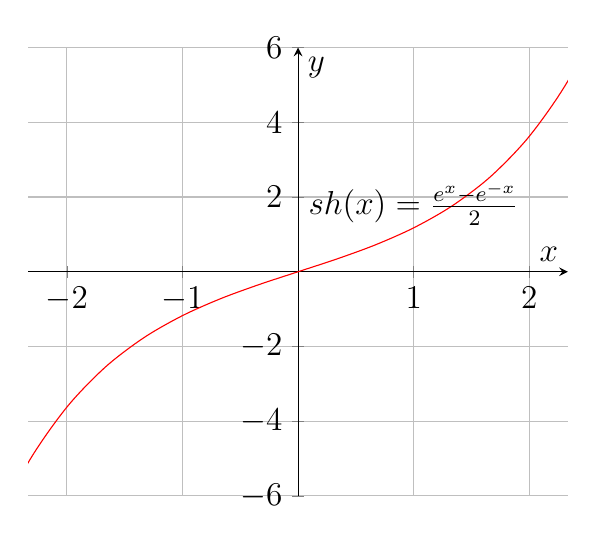
\begin{tikzpicture}
  \begin{axis}[domain=-4:4,ymin=-6,ymax=6, grid=both, font=\large, axis lines = middle, smooth, xlabel={$x$}, ylabel={$y$}]
    \addplot[draw=red] {(e^x - e^(-x)) / 2};
    \node at (axis cs:1,1.8) {$sh(x) = \frac{e^x - e^{-x}}{2}$};
  \end{axis}
\end{tikzpicture}

    \caption{$sh(x) = \frac{e^x - e^{-x}}{2}$}
    \label{sh_x}
\end{figure}

\subsubsection{双曲余弦}
\paragraph{}
$ch \, x = \frac{e^x + e^{-x}}{2}$

\begin{figure}[H]
  \centering
    % ch(x) = (e^x + e^(-x)) / 2
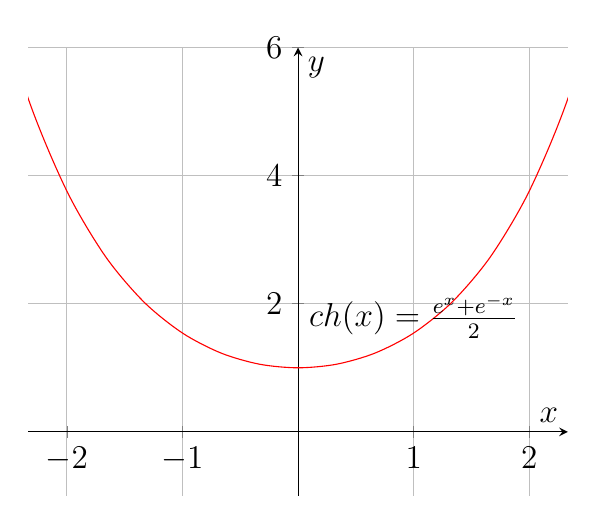
\begin{tikzpicture}
  \begin{axis}[domain=-4:4,ymin=-1,ymax=6, grid=both, font=\large, axis lines = middle, smooth, xlabel={$x$}, ylabel={$y$}]
    \addplot[draw=red] {(e^x + e^(-x)) / 2};
    \node at (axis cs:1,1.8) {$ch(x) = \frac{e^x + e^{-x}}{2}$};
  \end{axis}
\end{tikzpicture}

    \caption{$ch(x) = \frac{e^x + e^{-x}}{2}$}
    \label{ch_x}
\end{figure}

\subsubsection{双曲正切}
\paragraph{}
$th \, x = \frac{sh \, x}{ch \, x} = \frac{e^x - e^{-x}}{e^x + e^{-x}}$


\begin{figure}[H]
  \centering
    % th(x) = (e^x - e^(-x)) / (e^x -+e^(-x))
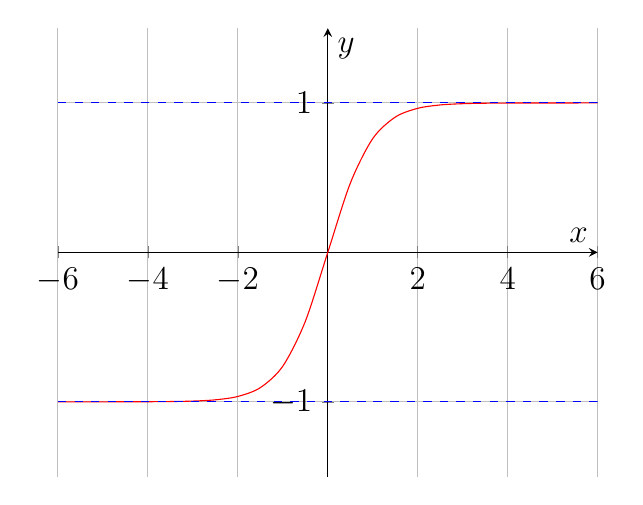
\begin{tikzpicture}
  \begin{axis}[domain=-6:6,ymin=-1.5,ymax=1.5, grid=both, font=\large, axis lines = middle, smooth, xlabel={$x$}, ylabel={$y$}]
    \addplot[draw=red] {(e^x - e^(-x)) / (e^x + e^(-x))};
    \addplot[dashed, draw=blue] {-1};
    \addplot[dashed, draw=blue] {1};
    \node at (axis cs:1,1.8) {$th(x) = \frac{e^x - e^{-x}}{e^x + e^{-x}}$};
  \end{axis}
\end{tikzpicture}

    \caption{$th(x) = \frac{e^x - e^{-x}}{e^x + e^{-x}}$}
    \label{th_x}
\end{figure}

\subsection{反双曲函数}
\subsubsection{反双曲正弦}
\paragraph{}
$y = arsh \, x = \ln(x + \sqrt{x^2 + 1})$

\begin{figure}[H]
  \centering
    % y = arsh(x)
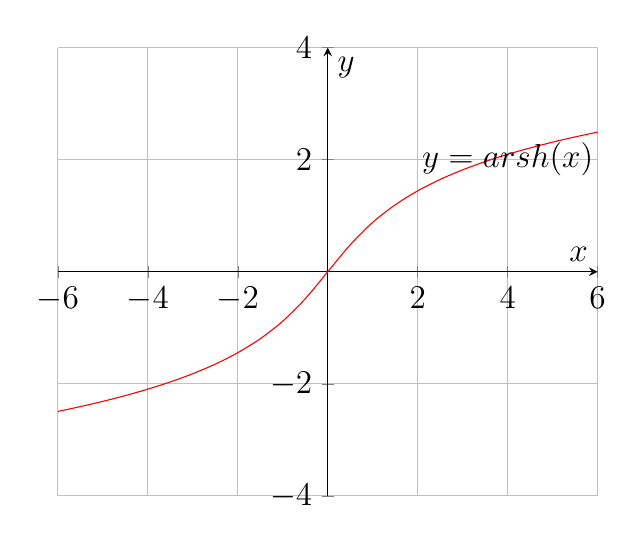
\begin{tikzpicture}
  \begin{axis}[domain=-6:6,ymin=-4,ymax=4, grid=both, font=\large, axis lines = middle, smooth, xlabel={$x$}, ylabel={$y$}]
    \addplot[draw=red] {ln(x + sqrt(x^2 + 1))};
    \node at (axis cs:4,2) {$y = arsh(x)$};
  \end{axis}
\end{tikzpicture}

    \caption{$y = arsh(x)$}
    \label{arsh_x}
\end{figure}

\subsubsection{反双曲余弦}
\paragraph{}
$y = arch \, x = \ln(x + \sqrt{x^2 - 1})$

\begin{figure}[H]
  \centering
    % y = arch(x)
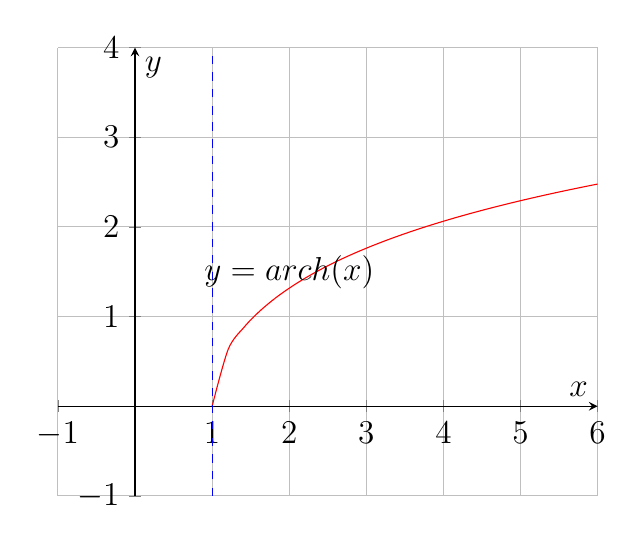
\begin{tikzpicture}
  \begin{axis}[xmin=-1, xmax=6,ymin=-1,ymax=4, grid=both, font=\large, axis lines = middle,
    smooth, xlabel={$x$}, ylabel={$y$}]
    \addplot[draw=red,domain=1:6] {ln(x + sqrt(x^2 - 1))};
    \addplot[dashed, draw=blue, mark=none] coordinates {(1, -1) (1, 4)};
    \node at (axis cs:2,1.5) {$y = arch(x)$};
  \end{axis}
\end{tikzpicture}

    \caption{$y = arch(x)$}
    \label{arch_x}
\end{figure}

\subsubsection{反双曲正切}
\paragraph{}
$y = arth \, x = \frac{1}{2} \ln(\frac{1 + x}{1 - x})$

\begin{figure}[H]
  \centering
    % y = arth(x)
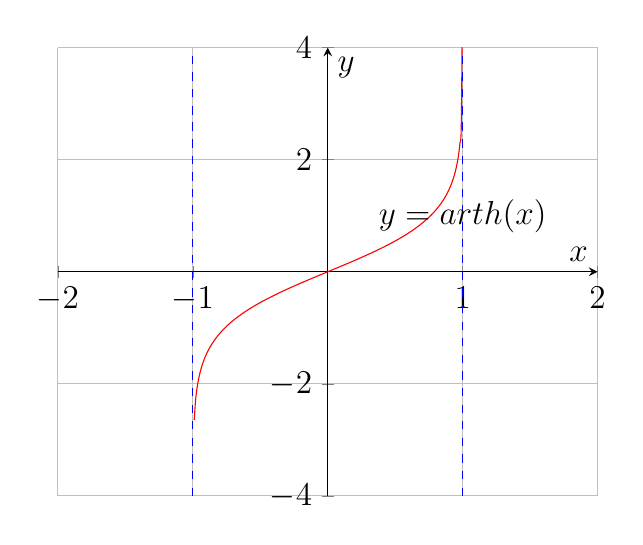
\begin{tikzpicture}
  \begin{axis}[xmin=-2,xmax=2,ymin=-4,ymax=4, grid=both, font=\large, axis lines=middle, smooth, xlabel={$x$}, ylabel={$y$}]
    \addplot[draw=red,domain=-1:1,samples=200] {(1/2)*ln((1 + x)/(1 - x))};
    \addplot[dashed, draw=blue, mark=none] coordinates {(1, -4) (1, 4)};
    \addplot[dashed, draw=blue, mark=none] coordinates {(-1, -4) (-1, 4)};
    \node at (axis cs:1,1) {$y = arth(x)$};
  \end{axis}
\end{tikzpicture}

    \caption{$y = arth(x)$}
    \label{arth_x}
\end{figure}

  \section{数列的极限}
    \subsection{数列}
\paragraph{}
如果按照某一法则,对每个$n \in N^+$,对应着一个确定的实数$x_n$,这些实数$x_n$按照下标$n$ 从小到大排序得到的一个序列,

\begin{equation}
x_1, x_2, x_3, ..., x_n, ...
\end{equation}

\paragraph{}
就叫数列,简记为数列 $\{x_n\}$。

\paragraph{}
$x_n$ 为一般项。

\subsection{数列极限}
\paragraph{}
设 $\{x_n\}$ 为一数列,如果存在常数 $a$,对于任意给定的正整数 $\varepsilon$(无论它多么小),总存在正整数 $N$ ,使得当 $n > N$ 时,不等式

\begin{equation}
|x_n - a| < \varepsilon,
\end{equation}

\paragraph{}
都成立,那么就称常数 $a$ 是数列 $\{x_n\}$ 的极限,或者称数列 $\{x_n\}$ 收敛于 $a$,记为

\begin{equation}
\lim_{n \to \infty} x_n = a,
\end{equation}

\paragraph{}
或

\begin{equation}
x_n \to a (n \to \infty).
\end{equation}

\paragraph{}
如果不存在这样的常数 $a$,就说数列 $\{x_n\}$ 是发散的。

\subsection{收敛数列的性质}
\subsubsection{极限的唯一性}
\paragraph{}
如果数列 $\{x_n\}$ 收敛,那么它的极限值唯一。

\subsubsection{收敛数列的有界性}
\paragraph{}
如果数列 $\{x_n\}$ 收敛,那么数列 $\{x_n\}$ 一定有界。

\subsubsection{收敛数列的保号性}
\paragraph{}
如果 $\displaystyle{\lim_{n \to \infty}} x_n = a$,且 $a > 0$(或 $a < 0$),那么存在正整数 $N > 0$,当 $n > N$ 时,都有 $x_n > 0$(或 $x_n < 0$)。

\subsubsection{收敛数列与其子数列间的关系}
\paragraph{}
如果数列 $\{x_n\}$ 收敛于 $a$,那么它的任一子数列也收敛,且极限也是 $a$。

  \section{函数的极限}
    \subsection{自变量趋于有限值时函数的极限}
\paragraph{}
设函数 $f(x)$ 在点 $x_0$ 的某一去心邻域内有定义,如果存在常数 $A$,对于任意给定的正数 $\varepsilon$(无论它多么小),总存在正数 $\delta$,使得当 $x$ 满足不等式 $0 < |x - x_0| < \delta$ 时,对应的函数值 $f(x)$ 都满足不等式

\begin{equation}
|f(x) - A| < \varepsilon,
\end{equation}

\paragraph{}
那么常数 $A$ 就叫做函数 $f(x)$ 当 $x \to x_0$ 时的极限,记作

\begin{equation}
\lim_{x \to x_0} f(x) = A,
\end{equation}

\paragraph{}
或

\begin{equation}
f(x) \to A(\text{当~~} x \to x_0).
\end{equation}

\subsubsection{单侧极限}
\paragraph{}
从 $x_0$ 的左侧或右侧趋近,即 $x_0 - \delta < x < x_0$ 或 $x_0 < x < x_0 + \delta$:

\begin{enumerate}
  \item 左极限:$\displaystyle{\lim_{x \to {x_0}^-}} f(x) = A \text{~~或~~} f({x_0}^-) = A$
  \item 右极限:$\displaystyle{\lim_{x \to {x_0}^+}} f(x) = A \text{~~或~~} f({x_0}^+) = A$
\end{enumerate}

\subsection{自变量趋于无穷大时函数的极限}
\paragraph{}
设函数 $f(x)$ 当 $|x|$ 大于某一正数时有定义,如果存在常数 $A$,对于任意给定的正整数 $\varepsilon$(无论它多么小),总存在着正数 $X$,使得当 $x$ 满足不等式 $|x| > X$ 时,对应的函数值 $f(x)$ 都满足不等式

\begin{equation}
|f(x) - A| < \varepsilon,
\end{equation}

\paragraph{}
那么常数 $A$ 就叫做函数 $f(x)$ 当 $x \to \infty$ 时的极限,记作

\begin{equation}
\lim_{x \to \infty} f(x) = A \text{~~或~~} f(x) \to A (\text{当~~} x \to \infty).
\end{equation}

\subsection{函数极限的性质}
\paragraph{}
下面的性质仅以 $\displaystyle{\lim_{x \to x_0}}f(x)$ 形式为代表给出的性质。

\subsubsection{函数极限的唯一性}
\paragraph{}
如果 $\displaystyle{\lim_{x \to x_0}}f(x)$ 存在,那么这极限唯一。

\subsubsection{函数极限的局部有界性}
\paragraph{}
如果 $\displaystyle{\lim_{x \to x_0}}f(x) = A$,那么存在常数 $M > 0$ 和 $\delta > 0$,使得当 $0 < |x - x_0| < \delta$ 时,有 $|f(x)| \leq M$.

\subsubsection{函数极限的局部保号性}
\paragraph{}
如果 $\displaystyle{\lim_{x \to x_0}}f(x) = A$,且 $A > 0 (\text{或~~} A < 0)$,那么存在常数 $\delta > 0$,使得当 $0 < |x - x_0| < \delta$ 时,有 $f(x) > 0 (\text{或~~} f(x) < 0)$。

\subsubsection{函数极限与数列极限的关系}
\paragraph{}
如果极限 $\displaystyle{\lim_{x \to x_0}}f(x)$ 存在,$\{x_n\}$ 为函数 $f(x)$ 的定义域内任一收敛于 $x_0$ 的数列,且满足 $x_n \neq x_0(n \in N^+)$,那么相应的函数值数列 $\{f(x_n)\}$ 必收敛,且 $\displaystyle{\lim_{n \to \infty}f(x_n) = \lim_{x \to x_0}f(x)}$。

  \section{无穷小与无穷大}
    \subsection{无穷小}
\paragraph{}
如果函数 $f(x)$ 当 $x \to x_0(\text{或~~} x \to \infty)$ 时的极限为零,那么称函数 $f(x)$ 为当 $x \to x_0(\text{或~~} x \to \infty)$ 时的无穷小。

\paragraph{}
无穷小与函数极限的关系:

\paragraph{}
\textbf{定理1} 在自变量的同一变化过程 $x \to x_0(\text{或~~} x \to \infty)$ 中,函数 $f(x)$ 具有极限 $A$ 的充分必要条件是 $f(x) = A + a$,其中 $a$ 是无穷小.

\subsection{无穷大}
\paragraph{}
设函数 $f(x )$ 在 $x_0$ 的某一去心邻域内有定义(或 $|x|$ 大于某一正数时有定义),如果对于任意给定的正数 $M$(无论它多么大),总存在正数 $\delta$(或正数 $X$),只要 $x$ 适合不等式 $0 < |x - x_0| < \delta (\text{或} |x| > X)$,对应的函数值 $f(x)$ 总满足不等式

\begin{equation}
|f(x)| > M,
\end{equation}

\paragraph{}
则称函数 $f(x)$ 为当 $x \to x_0(\text{或} x \to \infty)$ 时的无穷大,记作

\begin{gather}
\lim_{x \to x_0}f(x) = \infty \\
(\text{或} \lim_{x \to \infty}f(x) = \infty).
\end{gather}

\paragraph{}
正无穷大和负无穷大:

\begin{gather}
f(x) > M, \lim_{x \to x_0 (\text{或}x \to \infty)} f(x) = + \infty; \\
f(x) < - M, \lim_{x \to x_0 (\text{或}x \to \infty)} f(x) = - \infty.
\end{gather}

\paragraph{}
\textbf{定理2} 在自变量的同一变化过程中,如果 $f(x)$ 为无穷大,则 $\frac{1}{f(x)}$ 为无穷小;反之,如果 $f(x)$ 为无穷小,且 $f(x) \neq 0$,则 $\frac{1}{f(x)}$ 为无穷大.

  \section{极限运算法则}
    \subsection{定理}
\paragraph{}
以下结论适合 $x \to x_0 (\text{或} x \to \infty)$。

\subsubsection{定理1}
\paragraph{}
有限个无穷小的和也是无穷小。

\subsubsection{定理2}
\paragraph{}
有界函数与无穷小的乘积是无穷小。

\paragraph{}
\textbf{推论1} 常数与无穷小的乘积是无穷小。

\paragraph{}
\textbf{推论2} 有限个无穷小的乘积是无穷小.

\subsubsection{定理3}
\paragraph{}
如果 $\lim f(x) = A, \lim g(x) =B$,那么

\begin{enumerate}
  \item $\lim [f(x) \pm g(x)] = \lim f(x) \pm \lim g(x) = A \pm B$
  \item $\lim [f(x) \cdot g(x)] = \lim f(x) \cdot \lim g(x) = A \cdot B$
  \item 若 $B \neq 0$,则$\lim \frac{f(x)}{g(x)} = \frac{\lim f(x)}{\lim g(x)} = \frac{A}{B}$
\end{enumerate}

\paragraph{}
\textbf{推论1} 如果 $\lim f(x)$ 存在,而 $c$ 为常数,则 $\lim[cf(x)] = c \lim f(x)$。

\paragraph{}
\textbf{推论2} 如果 $\lim f(x)$ 存在,而 $n$ 是正整数,则 $\lim{[f(x)]}^n={[\lim f(x)]}^n$。

\subsubsection{定理4}
\paragraph{}
设有数列 $\{x_n\}$ 和 $\{y_n\}$,如果

\begin{equation}
\lim_{n \to \infty} x_n = A, \quad \lim_{n \to \infty} y_n = B
\end{equation}

\paragraph{}
那么

\begin{enumerate}
  \item $\displaystyle{\lim_{n \to \infty}(x_n \pm y_n) = A \pm B}$
  \item $\displaystyle{\lim_{n \to \infty}(x_n \cdot y_n) = A \cdot B}$
  \item 当 $y_n \neq 0 (n = 1, 2, ...)$ 且 $B \neq 0$ 时,$\displaystyle{\lim_{n \to \infty} \frac{x_n}{y_n}=\frac{A}{B}}$
\end{enumerate}

\subsubsection{定理5}
\paragraph{}
如果 $\varphi (x) \geq \psi (x)$,而 $\lim \varphi (x) = a, \lim \psi (x) = b$,那么 $a \geq b$。

\subsubsection{定理6 复合函数的极限运算法则}
\paragraph{}
设函数 $y = f[g(x)]$ 是由函数 $u = g(x)$ 与函数 $y = f(u)$ 复合而成,$f[g(x)]$ 在点 $x_0$ 的某去心邻域内有定义,若 $\displaystyle{\lim_{x \to x_0}g(x) = u_0, \lim_{u \to u_0} f(u) = A}$,且存在 $\delta_0 > 0$,当 $x \in \mathring{U}(x_0, \delta_0)$ 时,有 $g(x) \neq u_0$,则

\begin{equation}
\lim_{x \to x_0} f[g(x)] = \lim_{u \to u_0} f(u) = A  
\end{equation}

  \section{极限存在准则}
    \subsection{夹逼准则}
\paragraph{}
\textbf{准则1} 如果数列 $\{x_n\}$、$\{y_n\}$ 及 $\{z_n\}$ 满足下列条件:

\begin{enumerate}
  \item 从某项起,即 $\exists n_0 \in N$,当 $n > n_0$ 时,有 $y_n \leq x_n \leq z_n$
  \item $\displaystyle{\lim_{n \to \infty} y_n = a, \lim_{n \to \infty} z_n = a}$
\end{enumerate}

\paragraph{}
那么数列 $\{x_n\}$ 的极限存在,且 $\displaystyle{\lim_{n \to \infty} x_n = a}$。

\paragraph{}
\textbf{准则1} 如果

\begin{enumerate}
  \item 当 $x \in \mathring{U}(x_0, r)(\text{or~~}|x| > M)$ 时,$g(x) \leq f(x) \leq h(x)$
  \item $\displaystyle{\lim_{x \to x_0 (x \to \infty)} g(x) = A, \lim_{x \to x_0 (x \to \infty)} h(x) = A}$
\end{enumerate}

\paragraph{}
那么 $\displaystyle{\lim_{x \to x_0 (x \to \infty)} f(x)}$ 存在,且等于 $A$。

\subsection{单调有界数列必有极限}

\subsection{柯西极限存在准则}
\paragraph{}
数列 $\{x_n\}$ 收敛的充分必要条件是:对于任意给定的正数 $\varepsilon$,存在着这样的正整数 $N$,使得当 $m > N, n > N$ 时,就有 $|x_n - x_m| < \varepsilon$。

  \section{无穷小的比较}
    \paragraph{}
下面的 $\alpha$ 和 $\beta$ 都是同一个变量变化的过程的无穷小

\paragraph{}
如果 $\lim \frac{\beta}{\alpha} = 0$,就说 $\beta$ 是比 $\alpha$ 高阶的无穷小,记作 $\beta = o(\alpha)$;

\paragraph{}
如果 $\lim \frac{\beta}{\alpha} = \infty$,就说 $\beta$ 是比 $\alpha$ 低阶的无穷小;

\paragraph{}
如果 $\lim \frac{\beta}{\alpha} = c \neq 0$,就说 $\beta$ 与 $\alpha$ 是同阶无穷小;

\paragraph{}
如果 $\lim \frac{\beta}{\alpha^k} = c \neq 0, k > 0$,就说 $\beta$ 是关于 $\alpha$ 的 $k$ 阶无穷小;

\paragraph{}
如果 $\lim \frac{\beta}{\alpha} = 1$,就说 $\beta$ 与 $\alpha$ 是等价无穷小,记作 $\alpha \sim \beta$。

\paragraph{}
\textbf{定理1} $\beta$ 与 $\alpha$ 是等价无穷小的充分必要条件是 $\beta = \alpha + o(\alpha)$。

\paragraph{}
\textbf{定理2} 设 $\alpha \sim \alpha^\prime, \beta \sim \beta^\prime$,且 $\lim \frac{\beta^\prime}{\alpha^\prime}$ 存在,则 $\lim \frac{\beta}{\alpha} = lim \frac{\beta^\prime}{\alpha^\prime}$。

  \section{函数的连续性和间断点}
    \subsection{连续性}
\subsubsection{增量}
\paragraph{}
设变量 $u$ 从它的一个初值 $u_1$ 变到终值 $u_2$,终值与初值的差 $u_2 - u_1$ 就叫做变量 $u$ 的增量,记作 $\Delta u$,即

\begin{equation}
\Delta u = u_2 - u_1
\end{equation}

\paragraph{}
增量可以正,也可以负

\paragraph{}
$x$ 从 $x_0$ 变到 $x_0 + \Delta x$ 时,函数 $y$ 相应的从 $f(x_0)$ 变到 $f(x_0 + \Delta x)$,因此函数 $y$ 的增量为:

\begin{equation}
\Delta y = f(x_0 + \Delta x) - f(x_0)
\end{equation}

\subsubsection{连续性定义}
\paragraph{}
\textbf{定义:}设函数 $y = f(x)$ 在点 $x_0$ 的某一邻域内有定义,如果
\begin{gather}
\lim_{\Delta x \to 0}\Delta y = \lim_{\Delta x \to 0}[f(x_0 + \Delta x) - f(x_0)] = 0, \\
\text{或} \lim_{x \to x_0} f(x) = f(x_0).
\end{gather}

\paragraph{}
那么就称函数 $y = f(x)$ 在点 $x_0$ 连续。

\paragraph{}
\textbf{左连续:}如果 $\lim_{x \to x_0^-} f(x) = f(x_0^-)$ 存在且等于 $f(x_0)$,即

\begin{equation}
f(x_0^-) = f(x_0)
\end{equation}

\paragraph{}
\textbf{右连续:}如果 $\lim_{x \to x_0^+}f(x) = f(x_0^+)$ 存在且等于 $f(x_0)$,即

\begin{equation}
f(x_0^+) = f(x_0)
\end{equation}

\paragraph{}
在区间上每一点都连续的函数,叫做函数在该区间上连续。

\subsection{间断点}
\paragraph{}
设函数 $f(x)$ 在点 $x_0$ 的某去心邻域内有定义。在此前提,如果函数 $f(x)$ 有下列三种情形之一:

\begin{enumerate}
  \item 在 $x = x_0$ 没有定义
  \item 虽在 $x = x_0$ 有定义,但 $\lim_{x \to x_0}f(x)$ 不存在
  \item 前 2 点都成立,但 $\lim_{x \to x_0}f(x) \neq f(x_0)$
\end{enumerate}

\paragraph{}
则函数 $f(x)$ 在点 $x_0$ 为不连续,而点 $x_0$ 称为函数 $f(x)$ 的间断点。

  \section{连续函数的运算和初等函数的连续性}
    \subsection{连续函数的和、差、积、商的连续性}
\paragraph{}
\textbf{定理1:}设函数 $f(x)$ 和 $g(x)$ 在点 $x_0$ 连续,则它们的和(差)$f\pm g$ 、积 $f\cdot g$ 及商 $\frac{f}{g}(\text{当} g(x_0) \neq 0 \text{时})$ 都在点 $x_0$ 连续。

\subsection{反函数与复合函数的连续性}
\paragraph{}
\textbf{定理2:}如果函数 $y = f(x)$ 在区间 $I_x$ 上单调增加(或单调减少)且连续,那么它的反函数 $x = f^{-1}(y)$ 也对应的在区间 $I_y = \{y | y = f(x), x \in I_x\}$ 上单调增加(或单调减少)且连续。

\paragraph{}
\textbf{定理3:}设函数 $y = f[g(x)]$ 由函数 $u = g(x)$ 与函数 $y = f(u)$ 复合而成,$\mathring{U}(x_0) \subset D_{f \circ g}$,若 $\lim_{x \to x_0} g(x) = u_0$,而函数 $y = f(u)$ 在 $u = u_0$ 连续,则

\begin{equation}
\lim_{x \to x_0} f[g(x)] = \lim_{u \to u_0} f(u) = f(u_0).
\end{equation}

\paragraph{}
\textbf{定理4:}设函数 $y = f[g(x)]$ 是由函数 $u = g(x)$ 与函数 $y = f(u)$ 复合而成,$U(x_0) \subset D_{f \circ g}$,若函数 $u = g(x)$ 在 $x = x_0$ 连续,且 $g(x_0) = u_0$,而函数 $y = f(u)$ 在 $u = u_0$ 连续,则复合函数 $y = f[g(x)]$ 在 $x = x_0$ 也连续。

\subsection{初等函数的连续性}
\paragraph{}
初等函数在其定义域中都连续。

  \section{闭区间上连续函数的性质}
    \subsection{有界性与最大值最小值定理}
\paragraph{}
对于在区间 $I$ 上有定义的函数 $f(x)$,如果有 $x_0 \in I$,使得对于任一 $x \in I$ 都有

\begin{equation}
f(x) \leq f(x_0) (f(x) \geq f(x_0)),
\end{equation}

\paragraph{}
则称 $f(x_0)$ 是函数 $f(x)$ 在区间 $I$ 上的\textbf{最大值}(\textbf{最小值})。

\paragraph{}
\textbf{有界性与最大值最小值定理\;} 在闭区间上连续的函数在该区间上有界且一定能取得它的最大值和最小值。

\subsection{零点定理与介值定理}
\paragraph{}
\textbf{零点定理\;} 设函数 $f(x)$ 在闭区间 $[a,b]$ 上连续,且 $f(a)$ 与 $f(b)$ 异号(即 $f(a) \cdot f(b) < 0$),那么在开区间 $(a,b)$ 内至少有一点 $\xi$,使

\begin{equation}
f(\xi) = 0.
\end{equation}

\paragraph{}
\textbf{介值定理\;} 设函数 $f(x)$ 在闭区间 $[a,b]$ 上连续,且在这区间的端点取不同的函数值 $f(a) = A$ 及 $f(b) = B$,那么,对于 $A$ 与 $B$ 之间的任意一个数 $C$,在开区间 $(a,b)$ 内至少有一点 $\xi$,使得

\begin{equation}
f(\xi) = C (a < \xi < b).
\end{equation}

\paragraph{}
\textbf{推论\;} 在闭区间上连续的函数必取得介于最大值 $M$ 与最小值 $m$ 之间的任何值。

\subsection{一致连续性}
\paragraph{}
\textbf{定义\;} 设函数 $f(x)$ 在区间 $I$ 上有定义。如果对于任意给定的正数 $\varepsilon$,总存在着正数 $\delta$,使得对于区间 $I$ 上的任意两点 $x_1, x_2$,当 $|x_1 - x_2| < \delta$ 时,就有

\begin{equation}
|f(x_1) - f(x_2)| < \varepsilon,
\end{equation}

\paragraph{}
那么称函数 $f(x)$ 在区间 $I$ 上是一致性连续的。

\paragraph{}
\textbf{一致连续性定理\;} 如果函数 $f(x)$ 在闭区间 $[a,b]$ 上连续,那么它在该区间上一致连续。

\end{document}
